\documentclass[1p]{elsarticle_modified}
%\bibliographystyle{elsarticle-num}

%\usepackage[colorlinks]{hyperref}
%\usepackage{abbrmath_seonhwa} %\Abb, \Ascr, \Acal ,\Abf, \Afrak
\usepackage{amsfonts}
\usepackage{amssymb}
\usepackage{amsmath}
\usepackage{amsthm}
\usepackage{scalefnt}
\usepackage{amsbsy}
\usepackage{kotex}
\usepackage{caption}
\usepackage{subfig}
\usepackage{color}
\usepackage{graphicx}
\usepackage{xcolor} %% white, black, red, green, blue, cyan, magenta, yellow
\usepackage{float}
\usepackage{setspace}
\usepackage{hyperref}

\usepackage{tikz}
\usetikzlibrary{arrows}

\usepackage{multirow}
\usepackage{array} % fixed length table
\usepackage{hhline}

%%%%%%%%%%%%%%%%%%%%%
\makeatletter
\renewcommand*\env@matrix[1][\arraystretch]{%
	\edef\arraystretch{#1}%
	\hskip -\arraycolsep
	\let\@ifnextchar\new@ifnextchar
	\array{*\c@MaxMatrixCols c}}
\makeatother %https://tex.stackexchange.com/questions/14071/how-can-i-increase-the-line-spacing-in-a-matrix
%%%%%%%%%%%%%%%

\usepackage[normalem]{ulem}

\newcommand{\msout}[1]{\ifmmode\text{\sout{\ensuremath{#1}}}\else\sout{#1}\fi}
%SOURCE: \msout is \stkout macro in https://tex.stackexchange.com/questions/20609/strikeout-in-math-mode

\newcommand{\cancel}[1]{
	\ifmmode
	{\color{red}\msout{#1}}
	\else
	{\color{red}\sout{#1}}
	\fi
}

\newcommand{\add}[1]{
	{\color{blue}\uwave{#1}}
}

\newcommand{\replace}[2]{
	\ifmmode
	{\color{red}\msout{#1}}{\color{blue}\uwave{#2}}
	\else
	{\color{red}\sout{#1}}{\color{blue}\uwave{#2}}
	\fi
}

\newcommand{\Sol}{\mathcal{S}} %segment
\newcommand{\D}{D} %diagram
\newcommand{\A}{\mathcal{A}} %arc


%%%%%%%%%%%%%%%%%%%%%%%%%%%%%5 test

\def\sl{\operatorname{\textup{SL}}(2,\Cbb)}
\def\psl{\operatorname{\textup{PSL}}(2,\Cbb)}
\def\quan{\mkern 1mu \triangleright \mkern 1mu}

\theoremstyle{definition}
\newtheorem{thm}{Theorem}[section]
\newtheorem{prop}[thm]{Proposition}
\newtheorem{lem}[thm]{Lemma}
\newtheorem{ques}[thm]{Question}
\newtheorem{cor}[thm]{Corollary}
\newtheorem{defn}[thm]{Definition}
\newtheorem{exam}[thm]{Example}
\newtheorem{rmk}[thm]{Remark}
\newtheorem{alg}[thm]{Algorithm}

\newcommand{\I}{\sqrt{-1}}
\begin{document}

%\begin{frontmatter}
%
%\title{Boundary parabolic representations of knots up to 8 crossings}
%
%%% Group authors per affiliation:
%\author{Yunhi Cho} 
%\address{Department of Mathematics, University of Seoul, Seoul, Korea}
%\ead{yhcho@uos.ac.kr}
%
%
%\author{Seonhwa Kim} %\fnref{s_kim}}
%\address{Center for Geometry and Physics, Institute for Basic Science, Pohang, 37673, Korea}
%\ead{ryeona17@ibs.re.kr}
%
%\author{Hyuk Kim}
%\address{Department of Mathematical Sciences, Seoul National University, Seoul 08826, Korea}
%\ead{hyukkim@snu.ac.kr}
%
%\author{Seokbeom Yoon}
%\address{Department of Mathematical Sciences, Seoul National University, Seoul, 08826,  Korea}
%\ead{sbyoon15@snu.ac.kr}
%
%\begin{abstract}
%We find all boundary parabolic representation of knots up to 8 crossings.
%
%\end{abstract}
%\begin{keyword}
%    \MSC[2010] 57M25 
%\end{keyword}
%
%\end{frontmatter}

%\linenumbers
%\tableofcontents
%
\newcommand\colored[1]{\textcolor{white}{\rule[-0.35ex]{0.8em}{1.4ex}}\kern-0.8em\color{red} #1}%
%\newcommand\colored[1]{\textcolor{white}{ #1}\kern-2.17ex	\textcolor{white}{ #1}\kern-1.81ex	\textcolor{white}{ #1}\kern-2.15ex\color{red}#1	}

{\Large $\underline{12n_{0620}~(K12n_{0620})}$}

\setlength{\tabcolsep}{10pt}
\renewcommand{\arraystretch}{1.6}
\vspace{1cm}\begin{tabular}{m{100pt}>{\centering\arraybackslash}m{274pt}}
\multirow{5}{120pt}{
	\centering
	\includegraphics[width=112pt]{../../../GIT/diagram.site/Diagrams/png/2709_12n_0620.png}\\
\ \ \ A knot diagram\footnotemark}&
\allowdisplaybreaks
\textbf{Linearized knot diagam} \\
\cline{2-2}
 &
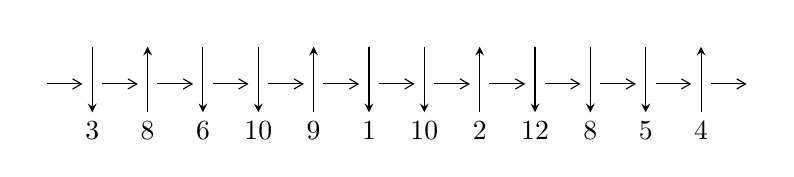
\begin{tikzpicture}[x=20pt, y=17pt]
	% nodes
	\node (C0) at (0, 0) {};
	\node (C1) at (1, 0) {};
	\node (C1U) at (1, +1) {};
	\node (C1D) at (1, -1) {3};

	\node (C2) at (2, 0) {};
	\node (C2U) at (2, +1) {};
	\node (C2D) at (2, -1) {8};

	\node (C3) at (3, 0) {};
	\node (C3U) at (3, +1) {};
	\node (C3D) at (3, -1) {6};

	\node (C4) at (4, 0) {};
	\node (C4U) at (4, +1) {};
	\node (C4D) at (4, -1) {10};

	\node (C5) at (5, 0) {};
	\node (C5U) at (5, +1) {};
	\node (C5D) at (5, -1) {9};

	\node (C6) at (6, 0) {};
	\node (C6U) at (6, +1) {};
	\node (C6D) at (6, -1) {1};

	\node (C7) at (7, 0) {};
	\node (C7U) at (7, +1) {};
	\node (C7D) at (7, -1) {10};

	\node (C8) at (8, 0) {};
	\node (C8U) at (8, +1) {};
	\node (C8D) at (8, -1) {2};

	\node (C9) at (9, 0) {};
	\node (C9U) at (9, +1) {};
	\node (C9D) at (9, -1) {12};

	\node (C10) at (10, 0) {};
	\node (C10U) at (10, +1) {};
	\node (C10D) at (10, -1) {8};

	\node (C11) at (11, 0) {};
	\node (C11U) at (11, +1) {};
	\node (C11D) at (11, -1) {5};

	\node (C12) at (12, 0) {};
	\node (C12U) at (12, +1) {};
	\node (C12D) at (12, -1) {4};
	\node (C13) at (13, 0) {};

	% arrows
	\draw[->,>={angle 60}]
	(C0) edge (C1) (C1) edge (C2) (C2) edge (C3) (C3) edge (C4) (C4) edge (C5) (C5) edge (C6) (C6) edge (C7) (C7) edge (C8) (C8) edge (C9) (C9) edge (C10) (C10) edge (C11) (C11) edge (C12) (C12) edge (C13) ;	\draw[->,>=stealth]
	(C1U) edge (C1D) (C2D) edge (C2U) (C3U) edge (C3D) (C4U) edge (C4D) (C5D) edge (C5U) (C6U) edge (C6D) (C7U) edge (C7D) (C8D) edge (C8U) (C9U) edge (C9D) (C10U) edge (C10D) (C11U) edge (C11D) (C12D) edge (C12U) ;
	\end{tikzpicture} \\
\hhline{~~} \\& 
\textbf{Solving Sequence} \\ \cline{2-2} 
 &
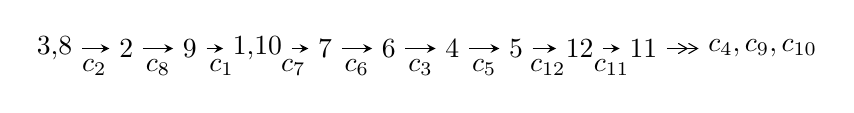
\begin{tikzpicture}[x=23pt, y=7pt]
	% node
	\node (A0) at (-1/8, 0) {3,8};
	\node (A1) at (1, 0) {2};
	\node (A2) at (2, 0) {9};
	\node (A3) at (49/16, 0) {1,10};
	\node (A4) at (33/8, 0) {7};
	\node (A5) at (41/8, 0) {6};
	\node (A6) at (49/8, 0) {4};
	\node (A7) at (57/8, 0) {5};
	\node (A8) at (65/8, 0) {12};
	\node (A9) at (73/8, 0) {11};
	\node (C1) at (1/2, -1) {$c_{2}$};
	\node (C2) at (3/2, -1) {$c_{8}$};
	\node (C3) at (5/2, -1) {$c_{1}$};
	\node (C4) at (29/8, -1) {$c_{7}$};
	\node (C5) at (37/8, -1) {$c_{6}$};
	\node (C6) at (45/8, -1) {$c_{3}$};
	\node (C7) at (53/8, -1) {$c_{5}$};
	\node (C8) at (61/8, -1) {$c_{12}$};
	\node (C9) at (69/8, -1) {$c_{11}$};
	\node (A10) at (11, 0) {$c_{4},c_{9},c_{10}$};

	% edge
	\draw[->,>=stealth]	
	(A0) edge (A1) (A1) edge (A2) (A2) edge (A3) (A3) edge (A4) (A4) edge (A5) (A5) edge (A6) (A6) edge (A7) (A7) edge (A8) (A8) edge (A9) ;
	\draw[->>,>={angle 60}]	
	(A9) edge (A10);
\end{tikzpicture} \\ 

\end{tabular} \\

\footnotetext{
The image of knot diagram is generated by the software ``\textbf{Draw programme}" developed by Andrew Bartholomew(\url{http://www.layer8.co.uk/maths/draw/index.htm\#Running-draw}), where we modified some parts for our purpose(\url{https://github.com/CATsTAILs/LinksPainter}).
}\phantom \\ \newline 
\centering \textbf{Ideals for irreducible components\footnotemark of $X_{\text{par}}$} 
 
\begin{align*}
I^u_{1}&=\langle 
-2.73681\times10^{256} u^{109}-4.05736\times10^{257} u^{108}+\cdots+1.53699\times10^{257} b-1.76787\times10^{260},\\
\phantom{I^u_{1}}&\phantom{= \langle  }1.94900\times10^{259} u^{109}-3.61458\times10^{259} u^{108}+\cdots+4.59560\times10^{259} a-9.14146\times10^{260},\\
\phantom{I^u_{1}}&\phantom{= \langle  }u^{110}-2 u^{109}+\cdots-963 u+299\rangle \\
I^u_{2}&=\langle 
11609161034 u^{38}+12620010667 u^{37}+\cdots+1705879031 b+52177194139,\\
\phantom{I^u_{2}}&\phantom{= \langle  }-15376761536 u^{38}-26045766200 u^{37}+\cdots+5117637093 a-26089510019,\\
\phantom{I^u_{2}}&\phantom{= \langle  }u^{39}+u^{38}+\cdots-5 u+3\rangle \\
\\
\end{align*}
\raggedright * 2 irreducible components of $\dim_{\mathbb{C}}=0$, with total 149 representations.\\
\footnotetext{All coefficients of polynomials are rational numbers. But the coefficients are sometimes approximated in decimal forms when there is not enough margin.}
\newpage
\renewcommand{\arraystretch}{1}
\centering \section*{I. $I^u_{1}= \langle -2.74\times10^{256} u^{109}-4.06\times10^{257} u^{108}+\cdots+1.54\times10^{257} b-1.77\times10^{260},\;1.95\times10^{259} u^{109}-3.61\times10^{259} u^{108}+\cdots+4.60\times10^{259} a-9.14\times10^{260},\;u^{110}-2 u^{109}+\cdots-963 u+299 \rangle$}
\flushleft \textbf{(i) Arc colorings}\\
\begin{tabular}{m{7pt} m{180pt} m{7pt} m{180pt} }
\flushright $a_{3}=$&$\begin{pmatrix}1\\0\end{pmatrix}$ \\
\flushright $a_{8}=$&$\begin{pmatrix}0\\u\end{pmatrix}$ \\
\flushright $a_{2}=$&$\begin{pmatrix}1\\u^2\end{pmatrix}$ \\
\flushright $a_{9}=$&$\begin{pmatrix}u\\u^3+u\end{pmatrix}$ \\
\flushright $a_{1}=$&$\begin{pmatrix}u^2+1\\u^2\end{pmatrix}$ \\
\flushright $a_{10}=$&$\begin{pmatrix}-0.424100 u^{109}+0.786531 u^{108}+\cdots-129.279 u+19.8918\\0.178063 u^{109}+2.63981 u^{108}+\cdots-2882.73 u+1150.21\end{pmatrix}$ \\
\flushright $a_{7}=$&$\begin{pmatrix}-0.353328 u^{109}+1.67139 u^{108}+\cdots-1477.43 u+519.669\\0.532410 u^{109}-2.28550 u^{108}+\cdots+1910.28 u-663.962\end{pmatrix}$ \\
\flushright $a_{6}=$&$\begin{pmatrix}-0.944196 u^{109}+2.84949 u^{108}+\cdots-2069.39 u+645.488\\0.965844 u^{109}-2.70003 u^{108}+\cdots+1777.43 u-527.622\end{pmatrix}$ \\
\flushright $a_{4}=$&$\begin{pmatrix}-0.721156 u^{109}+1.24858 u^{108}+\cdots-776.539 u+163.332\\0.969958 u^{109}-1.71452 u^{108}+\cdots+488.229 u+11.3660\end{pmatrix}$ \\
\flushright $a_{5}=$&$\begin{pmatrix}0.344268 u^{109}-0.0978060 u^{108}+\cdots-369.928 u+206.437\\1.24825 u^{109}-3.84301 u^{108}+\cdots+2734.98 u-855.933\end{pmatrix}$ \\
\flushright $a_{12}=$&$\begin{pmatrix}0.608160 u^{109}-0.734139 u^{108}+\cdots+154.268 u+49.4400\\0.366448 u^{109}-2.01607 u^{108}+\cdots+1749.68 u-629.644\end{pmatrix}$ \\
\flushright $a_{11}=$&$\begin{pmatrix}0.424100 u^{109}-0.786531 u^{108}+\cdots+129.279 u-19.8918\\-0.751274 u^{109}-1.98316 u^{108}+\cdots+2815.31 u-1168.65\end{pmatrix}$\\&\end{tabular}
\flushleft \textbf{(ii) Obstruction class $= -1$}\\~\\
\flushleft \textbf{(iii) Cusp Shapes $= 19.0742 u^{109}-31.2577 u^{108}+\cdots+11449.6 u-1567.00$}\\~\\
\newpage\renewcommand{\arraystretch}{1}
\flushleft \textbf{(iv) u-Polynomials at the component}\newline \\
\begin{tabular}{m{50pt}|m{274pt}}
Crossings & \hspace{64pt}u-Polynomials at each crossing \\
\hline $$\begin{aligned}c_{1}\end{aligned}$$&$\begin{aligned}
&u^{110}+42 u^{109}+\cdots+4187325 u+89401
\end{aligned}$\\
\hline $$\begin{aligned}c_{2},c_{8}\end{aligned}$$&$\begin{aligned}
&u^{110}+2 u^{109}+\cdots+963 u+299
\end{aligned}$\\
\hline $$\begin{aligned}c_{3}\end{aligned}$$&$\begin{aligned}
&u^{110}+10 u^{109}+\cdots+25 u-1
\end{aligned}$\\
\hline $$\begin{aligned}c_{4}\end{aligned}$$&$\begin{aligned}
&u^{110}+8 u^{108}+\cdots+1099616 u+270272
\end{aligned}$\\
\hline $$\begin{aligned}c_{5}\end{aligned}$$&$\begin{aligned}
&u^{110}-3 u^{109}+\cdots+9806561 u+1029481
\end{aligned}$\\
\hline $$\begin{aligned}c_{6}\end{aligned}$$&$\begin{aligned}
&u^{110}+5 u^{109}+\cdots+140122 u-5273
\end{aligned}$\\
\hline $$\begin{aligned}c_{7},c_{10}\end{aligned}$$&$\begin{aligned}
&u^{110}+u^{109}+\cdots+26 u+1
\end{aligned}$\\
\hline $$\begin{aligned}c_{9}\end{aligned}$$&$\begin{aligned}
&u^{110}-7 u^{109}+\cdots-40 u+1
\end{aligned}$\\
\hline $$\begin{aligned}c_{11}\end{aligned}$$&$\begin{aligned}
&u^{110}+3 u^{109}+\cdots+54488131 u+3556907
\end{aligned}$\\
\hline $$\begin{aligned}c_{12}\end{aligned}$$&$\begin{aligned}
&u^{110}+8 u^{109}+\cdots-5432 u+83
\end{aligned}$\\
\hline
\end{tabular}\\~\\
\newpage\renewcommand{\arraystretch}{1}
\flushleft \textbf{(v) Riley Polynomials at the component}\newline \\
\begin{tabular}{m{50pt}|m{274pt}}
Crossings & \hspace{64pt}Riley Polynomials at each crossing \\
\hline $$\begin{aligned}c_{1}\end{aligned}$$&$\begin{aligned}
&y^{110}+62 y^{109}+\cdots-1749078882747 y+7992538801
\end{aligned}$\\
\hline $$\begin{aligned}c_{2},c_{8}\end{aligned}$$&$\begin{aligned}
&y^{110}+42 y^{109}+\cdots+4187325 y+89401
\end{aligned}$\\
\hline $$\begin{aligned}c_{3}\end{aligned}$$&$\begin{aligned}
&y^{110}-24 y^{109}+\cdots-35 y+1
\end{aligned}$\\
\hline $$\begin{aligned}c_{4}\end{aligned}$$&$\begin{aligned}
&y^{110}+16 y^{109}+\cdots+4786463564800 y+73046953984
\end{aligned}$\\
\hline $$\begin{aligned}c_{5}\end{aligned}$$&$\begin{aligned}
&y^{110}-29 y^{109}+\cdots-26980827938145 y+1059831129361
\end{aligned}$\\
\hline $$\begin{aligned}c_{6}\end{aligned}$$&$\begin{aligned}
&y^{110}+45 y^{109}+\cdots-976149500 y+27804529
\end{aligned}$\\
\hline $$\begin{aligned}c_{7},c_{10}\end{aligned}$$&$\begin{aligned}
&y^{110}+87 y^{109}+\cdots+98 y+1
\end{aligned}$\\
\hline $$\begin{aligned}c_{9}\end{aligned}$$&$\begin{aligned}
&y^{110}-27 y^{109}+\cdots-484 y+1
\end{aligned}$\\
\hline $$\begin{aligned}c_{11}\end{aligned}$$&$\begin{aligned}
&y^{110}+23 y^{109}+\cdots-545838580976069 y+12651587406649
\end{aligned}$\\
\hline $$\begin{aligned}c_{12}\end{aligned}$$&$\begin{aligned}
&y^{110}-6 y^{109}+\cdots-29183256 y+6889
\end{aligned}$\\
\hline
\end{tabular}\\~\\
\newpage\flushleft \textbf{(vi) Complex Volumes and Cusp Shapes}
$$\begin{array}{c|c|c}  
\text{Solutions to }I^u_{1}& \I (\text{vol} + \sqrt{-1}CS) & \text{Cusp shape}\\
 \hline 
\begin{aligned}
u &= -0.722846 + 0.701707 I \\
a &= -1.017860 - 0.590067 I \\
b &= -0.727453 - 0.080952 I\end{aligned}
 & \phantom{-}3.33089 - 2.04230 I & \phantom{-0.000000 } 0 \\ \hline\begin{aligned}
u &= -0.722846 - 0.701707 I \\
a &= -1.017860 + 0.590067 I \\
b &= -0.727453 + 0.080952 I\end{aligned}
 & \phantom{-}3.33089 + 2.04230 I & \phantom{-0.000000 } 0 \\ \hline\begin{aligned}
u &= \phantom{-}0.445918 + 0.876034 I \\
a &= \phantom{-}0.58584 - 1.30472 I \\
b &= \phantom{-}1.41639 - 0.62868 I\end{aligned}
 & -6.18417 + 2.12923 I & \phantom{-0.000000 } 0 \\ \hline\begin{aligned}
u &= \phantom{-}0.445918 - 0.876034 I \\
a &= \phantom{-}0.58584 + 1.30472 I \\
b &= \phantom{-}1.41639 + 0.62868 I\end{aligned}
 & -6.18417 - 2.12923 I & \phantom{-0.000000 } 0 \\ \hline\begin{aligned}
u &= -0.698901 + 0.679034 I \\
a &= \phantom{-}0.90817 - 1.27666 I \\
b &= -0.86504 - 2.14123 I\end{aligned}
 & \phantom{-}3.33911 + 2.19870 I & \phantom{-0.000000 } 0 \\ \hline\begin{aligned}
u &= -0.698901 - 0.679034 I \\
a &= \phantom{-}0.90817 + 1.27666 I \\
b &= -0.86504 + 2.14123 I\end{aligned}
 & \phantom{-}3.33911 - 2.19870 I & \phantom{-0.000000 } 0 \\ \hline\begin{aligned}
u &= -0.346243 + 0.975342 I \\
a &= -0.413122 + 0.497225 I \\
b &= \phantom{-}0.006959 + 0.697219 I\end{aligned}
 & -0.60914 - 1.80163 I & \phantom{-0.000000 } 0 \\ \hline\begin{aligned}
u &= -0.346243 - 0.975342 I \\
a &= -0.413122 - 0.497225 I \\
b &= \phantom{-}0.006959 - 0.697219 I\end{aligned}
 & -0.60914 + 1.80163 I & \phantom{-0.000000 } 0 \\ \hline\begin{aligned}
u &= \phantom{-}0.763827 + 0.726239 I \\
a &= -1.59712 - 0.66520 I \\
b &= \phantom{-}0.18657 - 1.56551 I\end{aligned}
 & \phantom{-}7.19825 - 4.32425 I & \phantom{-0.000000 } 0 \\ \hline\begin{aligned}
u &= \phantom{-}0.763827 - 0.726239 I \\
a &= -1.59712 + 0.66520 I \\
b &= \phantom{-}0.18657 + 1.56551 I\end{aligned}
 & \phantom{-}7.19825 + 4.32425 I & \phantom{-0.000000 } 0\\
 \hline 
 \end{array}$$\newpage$$\begin{array}{c|c|c}  
\text{Solutions to }I^u_{1}& \I (\text{vol} + \sqrt{-1}CS) & \text{Cusp shape}\\
 \hline 
\begin{aligned}
u &= \phantom{-}0.571377 + 0.750356 I \\
a &= -0.769118 + 0.584129 I \\
b &= \phantom{-}0.216929 + 0.253116 I\end{aligned}
 & -1.84127 - 0.70860 I & \phantom{-0.000000 } 0 \\ \hline\begin{aligned}
u &= \phantom{-}0.571377 - 0.750356 I \\
a &= -0.769118 - 0.584129 I \\
b &= \phantom{-}0.216929 - 0.253116 I\end{aligned}
 & -1.84127 + 0.70860 I & \phantom{-0.000000 } 0 \\ \hline\begin{aligned}
u &= \phantom{-}0.595378 + 0.874733 I \\
a &= \phantom{-}0.177994 - 1.026400 I \\
b &= \phantom{-}0.43318 - 1.54478 I\end{aligned}
 & -2.04500 + 5.27108 I & \phantom{-0.000000 } 0 \\ \hline\begin{aligned}
u &= \phantom{-}0.595378 - 0.874733 I \\
a &= \phantom{-}0.177994 + 1.026400 I \\
b &= \phantom{-}0.43318 + 1.54478 I\end{aligned}
 & -2.04500 - 5.27108 I & \phantom{-0.000000 } 0 \\ \hline\begin{aligned}
u &= -0.626457 + 0.864050 I \\
a &= \phantom{-}1.14154 - 0.95416 I \\
b &= -0.96129 - 2.66223 I\end{aligned}
 & \phantom{-}2.41221 - 2.45417 I & \phantom{-0.000000 } 0 \\ \hline\begin{aligned}
u &= -0.626457 - 0.864050 I \\
a &= \phantom{-}1.14154 + 0.95416 I \\
b &= -0.96129 + 2.66223 I\end{aligned}
 & \phantom{-}2.41221 + 2.45417 I & \phantom{-0.000000 } 0 \\ \hline\begin{aligned}
u &= \phantom{-}0.337405 + 0.860809 I \\
a &= \phantom{-}0.545050 - 0.680241 I \\
b &= \phantom{-}1.90211 - 0.19509 I\end{aligned}
 & -3.62539 - 1.21292 I & \phantom{-0.000000 } 0 \\ \hline\begin{aligned}
u &= \phantom{-}0.337405 - 0.860809 I \\
a &= \phantom{-}0.545050 + 0.680241 I \\
b &= \phantom{-}1.90211 + 0.19509 I\end{aligned}
 & -3.62539 + 1.21292 I & \phantom{-0.000000 } 0 \\ \hline\begin{aligned}
u &= \phantom{-}0.002367 + 0.923336 I \\
a &= \phantom{-}1.198900 - 0.401062 I \\
b &= \phantom{-}1.352370 - 0.092461 I\end{aligned}
 & \phantom{-}1.97943 - 4.96044 I & \phantom{-0.000000 } 0 \\ \hline\begin{aligned}
u &= \phantom{-}0.002367 - 0.923336 I \\
a &= \phantom{-}1.198900 + 0.401062 I \\
b &= \phantom{-}1.352370 + 0.092461 I\end{aligned}
 & \phantom{-}1.97943 + 4.96044 I & \phantom{-0.000000 } 0\\
 \hline 
 \end{array}$$\newpage$$\begin{array}{c|c|c}  
\text{Solutions to }I^u_{1}& \I (\text{vol} + \sqrt{-1}CS) & \text{Cusp shape}\\
 \hline 
\begin{aligned}
u &= \phantom{-}0.362094 + 1.020900 I \\
a &= -0.431256 + 0.237298 I \\
b &= \phantom{-}0.677429 + 0.253537 I\end{aligned}
 & -1.86815 - 0.95241 I & \phantom{-0.000000 } 0 \\ \hline\begin{aligned}
u &= \phantom{-}0.362094 - 1.020900 I \\
a &= -0.431256 - 0.237298 I \\
b &= \phantom{-}0.677429 - 0.253537 I\end{aligned}
 & -1.86815 + 0.95241 I & \phantom{-0.000000 } 0 \\ \hline\begin{aligned}
u &= \phantom{-}1.09151\phantom{ +0.000000I} \\
a &= -1.20966\phantom{ +0.000000I} \\
b &= \phantom{-}0.426400\phantom{ +0.000000I}\end{aligned}
 & -2.72278\phantom{ +0.000000I} & \phantom{-0.000000 } 0 \\ \hline\begin{aligned}
u &= \phantom{-}0.156976 + 0.886403 I \\
a &= \phantom{-}0.517031 - 0.819311 I \\
b &= -2.20512 - 1.12750 I\end{aligned}
 & -5.39558 + 5.25843 I & \phantom{-0.000000 } 0 \\ \hline\begin{aligned}
u &= \phantom{-}0.156976 - 0.886403 I \\
a &= \phantom{-}0.517031 + 0.819311 I \\
b &= -2.20512 + 1.12750 I\end{aligned}
 & -5.39558 - 5.25843 I & \phantom{-0.000000 } 0 \\ \hline\begin{aligned}
u &= -0.704749 + 0.860618 I \\
a &= -1.10219 + 0.90580 I \\
b &= \phantom{-}1.22696 + 2.04135 I\end{aligned}
 & \phantom{-}6.18973 - 6.69907 I & \phantom{-0.000000 } 0 \\ \hline\begin{aligned}
u &= -0.704749 - 0.860618 I \\
a &= -1.10219 - 0.90580 I \\
b &= \phantom{-}1.22696 - 2.04135 I\end{aligned}
 & \phantom{-}6.18973 + 6.69907 I & \phantom{-0.000000 } 0 \\ \hline\begin{aligned}
u &= \phantom{-}0.703019 + 0.866531 I \\
a &= \phantom{-}0.410291 - 0.025373 I \\
b &= -1.26321 - 0.79273 I\end{aligned}
 & -2.06981 + 6.66278 I & \phantom{-0.000000 } 0 \\ \hline\begin{aligned}
u &= \phantom{-}0.703019 - 0.866531 I \\
a &= \phantom{-}0.410291 + 0.025373 I \\
b &= -1.26321 + 0.79273 I\end{aligned}
 & -2.06981 - 6.66278 I & \phantom{-0.000000 } 0 \\ \hline\begin{aligned}
u &= \phantom{-}0.440379 + 0.763170 I \\
a &= -0.64807 + 1.58057 I \\
b &= -1.141980 + 0.190483 I\end{aligned}
 & -5.80700 + 1.50471 I & \phantom{-0.000000 } 0\\
 \hline 
 \end{array}$$\newpage$$\begin{array}{c|c|c}  
\text{Solutions to }I^u_{1}& \I (\text{vol} + \sqrt{-1}CS) & \text{Cusp shape}\\
 \hline 
\begin{aligned}
u &= \phantom{-}0.440379 - 0.763170 I \\
a &= -0.64807 - 1.58057 I \\
b &= -1.141980 - 0.190483 I\end{aligned}
 & -5.80700 - 1.50471 I & \phantom{-0.000000 } 0 \\ \hline\begin{aligned}
u &= \phantom{-}0.804886 + 0.781354 I \\
a &= \phantom{-}1.35580 + 0.79298 I \\
b &= -0.33866 + 1.71063 I\end{aligned}
 & \phantom{-}7.48927 + 1.66053 I & \phantom{-0.000000 } 0 \\ \hline\begin{aligned}
u &= \phantom{-}0.804886 - 0.781354 I \\
a &= \phantom{-}1.35580 - 0.79298 I \\
b &= -0.33866 - 1.71063 I\end{aligned}
 & \phantom{-}7.48927 - 1.66053 I & \phantom{-0.000000 } 0 \\ \hline\begin{aligned}
u &= -0.856105 + 0.734749 I \\
a &= \phantom{-}1.17022 + 0.96909 I \\
b &= \phantom{-}1.012480 + 0.338174 I\end{aligned}
 & \phantom{-}1.48996 + 3.88010 I & \phantom{-0.000000 } 0 \\ \hline\begin{aligned}
u &= -0.856105 - 0.734749 I \\
a &= \phantom{-}1.17022 - 0.96909 I \\
b &= \phantom{-}1.012480 - 0.338174 I\end{aligned}
 & \phantom{-}1.48996 - 3.88010 I & \phantom{-0.000000 } 0 \\ \hline\begin{aligned}
u &= -0.150463 + 1.124600 I \\
a &= -1.031350 + 0.040889 I \\
b &= \phantom{-}0.215838 + 0.240483 I\end{aligned}
 & -1.23331 + 1.22688 I & \phantom{-0.000000 } 0 \\ \hline\begin{aligned}
u &= -0.150463 - 1.124600 I \\
a &= -1.031350 - 0.040889 I \\
b &= \phantom{-}0.215838 - 0.240483 I\end{aligned}
 & -1.23331 - 1.22688 I & \phantom{-0.000000 } 0 \\ \hline\begin{aligned}
u &= -0.719221 + 0.878314 I \\
a &= -0.907622 + 0.945954 I \\
b &= \phantom{-}0.35687 + 2.59585 I\end{aligned}
 & \phantom{-}6.14126 + 1.24957 I & \phantom{-0.000000 } 0 \\ \hline\begin{aligned}
u &= -0.719221 - 0.878314 I \\
a &= -0.907622 - 0.945954 I \\
b &= \phantom{-}0.35687 - 2.59585 I\end{aligned}
 & \phantom{-}6.14126 - 1.24957 I & \phantom{-0.000000 } 0 \\ \hline\begin{aligned}
u &= -0.296758 + 0.812163 I \\
a &= -1.257690 + 0.297788 I \\
b &= -0.518619 - 0.150423 I\end{aligned}
 & \phantom{-}0.537031 - 1.207440 I & \phantom{-0.000000 } 0\\
 \hline 
 \end{array}$$\newpage$$\begin{array}{c|c|c}  
\text{Solutions to }I^u_{1}& \I (\text{vol} + \sqrt{-1}CS) & \text{Cusp shape}\\
 \hline 
\begin{aligned}
u &= -0.296758 - 0.812163 I \\
a &= -1.257690 - 0.297788 I \\
b &= -0.518619 + 0.150423 I\end{aligned}
 & \phantom{-}0.537031 + 1.207440 I & \phantom{-0.000000 } 0 \\ \hline\begin{aligned}
u &= \phantom{-}0.997006 + 0.556264 I \\
a &= \phantom{-}1.19356 + 0.90160 I \\
b &= -0.43208 + 1.57023 I\end{aligned}
 & \phantom{-}8.27801 - 4.57132 I & \phantom{-0.000000 } 0 \\ \hline\begin{aligned}
u &= \phantom{-}0.997006 - 0.556264 I \\
a &= \phantom{-}1.19356 - 0.90160 I \\
b &= -0.43208 - 1.57023 I\end{aligned}
 & \phantom{-}8.27801 + 4.57132 I & \phantom{-0.000000 } 0 \\ \hline\begin{aligned}
u &= \phantom{-}0.400337 + 1.070610 I \\
a &= \phantom{-}0.130198 + 0.182402 I \\
b &= -0.139502 - 0.845139 I\end{aligned}
 & -4.28944 + 3.55197 I & \phantom{-0.000000 } 0 \\ \hline\begin{aligned}
u &= \phantom{-}0.400337 - 1.070610 I \\
a &= \phantom{-}0.130198 - 0.182402 I \\
b &= -0.139502 + 0.845139 I\end{aligned}
 & -4.28944 - 3.55197 I & \phantom{-0.000000 } 0 \\ \hline\begin{aligned}
u &= \phantom{-}0.256791 + 0.805667 I \\
a &= \phantom{-}0.464107 + 1.205970 I \\
b &= -1.098290 + 0.008504 I\end{aligned}
 & -3.53626 + 3.81291 I & \phantom{-0.000000 } 0 \\ \hline\begin{aligned}
u &= \phantom{-}0.256791 - 0.805667 I \\
a &= \phantom{-}0.464107 - 1.205970 I \\
b &= -1.098290 - 0.008504 I\end{aligned}
 & -3.53626 - 3.81291 I & \phantom{-0.000000 } 0 \\ \hline\begin{aligned}
u &= \phantom{-}0.281043 + 1.129070 I \\
a &= \phantom{-}0.0542065 + 0.1136410 I \\
b &= \phantom{-}0.136152 - 0.267958 I\end{aligned}
 & -5.24948 - 0.28210 I & \phantom{-0.000000 } 0 \\ \hline\begin{aligned}
u &= \phantom{-}0.281043 - 1.129070 I \\
a &= \phantom{-}0.0542065 - 0.1136410 I \\
b &= \phantom{-}0.136152 + 0.267958 I\end{aligned}
 & -5.24948 + 0.28210 I & \phantom{-0.000000 } 0 \\ \hline\begin{aligned}
u &= -0.849507 + 0.809289 I \\
a &= -0.741868 + 1.083740 I \\
b &= \phantom{-}0.40181 + 2.05841 I\end{aligned}
 & \phantom{-}3.63531 + 1.33713 I & \phantom{-0.000000 } 0\\
 \hline 
 \end{array}$$\newpage$$\begin{array}{c|c|c}  
\text{Solutions to }I^u_{1}& \I (\text{vol} + \sqrt{-1}CS) & \text{Cusp shape}\\
 \hline 
\begin{aligned}
u &= -0.849507 - 0.809289 I \\
a &= -0.741868 - 1.083740 I \\
b &= \phantom{-}0.40181 - 2.05841 I\end{aligned}
 & \phantom{-}3.63531 - 1.33713 I & \phantom{-0.000000 } 0 \\ \hline\begin{aligned}
u &= -0.292829 + 1.140030 I \\
a &= -1.180480 + 0.389242 I \\
b &= -1.46797 + 0.39561 I\end{aligned}
 & -0.137879 + 0.321132 I & \phantom{-0.000000 } 0 \\ \hline\begin{aligned}
u &= -0.292829 - 1.140030 I \\
a &= -1.180480 - 0.389242 I \\
b &= -1.46797 - 0.39561 I\end{aligned}
 & -0.137879 - 0.321132 I & \phantom{-0.000000 } 0 \\ \hline\begin{aligned}
u &= \phantom{-}1.024800 + 0.580684 I \\
a &= -1.19370 - 1.00233 I \\
b &= \phantom{-}0.34345 - 1.67474 I\end{aligned}
 & \phantom{-}7.2811 - 12.3035 I & \phantom{-0.000000 } 0 \\ \hline\begin{aligned}
u &= \phantom{-}1.024800 - 0.580684 I \\
a &= -1.19370 + 1.00233 I \\
b &= \phantom{-}0.34345 + 1.67474 I\end{aligned}
 & \phantom{-}7.2811 + 12.3035 I & \phantom{-0.000000 } 0 \\ \hline\begin{aligned}
u &= \phantom{-}0.749698 + 0.289214 I \\
a &= -0.1297850 + 0.0239455 I \\
b &= \phantom{-}0.240853 + 0.119770 I\end{aligned}
 & -0.98667 - 3.24837 I & \phantom{-0.000000 } 0 \\ \hline\begin{aligned}
u &= \phantom{-}0.749698 - 0.289214 I \\
a &= -0.1297850 - 0.0239455 I \\
b &= \phantom{-}0.240853 - 0.119770 I\end{aligned}
 & -0.98667 + 3.24837 I & \phantom{-0.000000 } 0 \\ \hline\begin{aligned}
u &= -1.054500 + 0.566130 I \\
a &= \phantom{-}0.537611 - 1.194650 I \\
b &= -0.55155 - 1.70109 I\end{aligned}
 & \phantom{-}8.01631 + 1.94598 I & \phantom{-0.000000 } 0 \\ \hline\begin{aligned}
u &= -1.054500 - 0.566130 I \\
a &= \phantom{-}0.537611 + 1.194650 I \\
b &= -0.55155 + 1.70109 I\end{aligned}
 & \phantom{-}8.01631 - 1.94598 I & \phantom{-0.000000 } 0 \\ \hline\begin{aligned}
u &= -0.677358 + 0.988928 I \\
a &= \phantom{-}0.631718 + 0.861883 I \\
b &= \phantom{-}0.957361 + 0.484007 I\end{aligned}
 & \phantom{-}2.45837 - 3.33905 I & \phantom{-0.000000 } 0\\
 \hline 
 \end{array}$$\newpage$$\begin{array}{c|c|c}  
\text{Solutions to }I^u_{1}& \I (\text{vol} + \sqrt{-1}CS) & \text{Cusp shape}\\
 \hline 
\begin{aligned}
u &= -0.677358 - 0.988928 I \\
a &= \phantom{-}0.631718 - 0.861883 I \\
b &= \phantom{-}0.957361 - 0.484007 I\end{aligned}
 & \phantom{-}2.45837 + 3.33905 I & \phantom{-0.000000 } 0 \\ \hline\begin{aligned}
u &= \phantom{-}0.222666 + 0.768558 I \\
a &= -0.777803 + 0.666985 I \\
b &= \phantom{-}2.96488 + 0.93575 I\end{aligned}
 & -4.79949 - 3.56029 I & \phantom{-0.000000 } 0 \\ \hline\begin{aligned}
u &= \phantom{-}0.222666 - 0.768558 I \\
a &= -0.777803 - 0.666985 I \\
b &= \phantom{-}2.96488 - 0.93575 I\end{aligned}
 & -4.79949 + 3.56029 I & \phantom{-0.000000 } 0 \\ \hline\begin{aligned}
u &= \phantom{-}0.567412 + 1.059780 I \\
a &= \phantom{-}0.0499061 - 0.1307740 I \\
b &= -0.765301 + 0.192801 I\end{aligned}
 & \phantom{-}0.04110 + 7.67997 I & \phantom{-0.000000 } 0 \\ \hline\begin{aligned}
u &= \phantom{-}0.567412 - 1.059780 I \\
a &= \phantom{-}0.0499061 + 0.1307740 I \\
b &= -0.765301 - 0.192801 I\end{aligned}
 & \phantom{-}0.04110 - 7.67997 I & \phantom{-0.000000 } 0 \\ \hline\begin{aligned}
u &= -0.522752 + 1.085990 I \\
a &= \phantom{-}0.973408 - 0.524333 I \\
b &= \phantom{-}1.46745 - 1.79487 I\end{aligned}
 & \phantom{-}1.33546 - 7.85597 I & \phantom{-0.000000 } 0 \\ \hline\begin{aligned}
u &= -0.522752 - 1.085990 I \\
a &= \phantom{-}0.973408 + 0.524333 I \\
b &= \phantom{-}1.46745 + 1.79487 I\end{aligned}
 & \phantom{-}1.33546 + 7.85597 I & \phantom{-0.000000 } 0 \\ \hline\begin{aligned}
u &= -0.667948 + 1.003410 I \\
a &= \phantom{-}1.104430 - 0.758801 I \\
b &= -0.58229 - 2.28353 I\end{aligned}
 & \phantom{-}2.34844 - 7.49528 I & \phantom{-0.000000 } 0 \\ \hline\begin{aligned}
u &= -0.667948 - 1.003410 I \\
a &= \phantom{-}1.104430 + 0.758801 I \\
b &= -0.58229 + 2.28353 I\end{aligned}
 & \phantom{-}2.34844 + 7.49528 I & \phantom{-0.000000 } 0 \\ \hline\begin{aligned}
u &= \phantom{-}0.703432 + 0.982255 I \\
a &= -0.57713 - 1.34466 I \\
b &= \phantom{-}0.71275 - 2.41009 I\end{aligned}
 & \phantom{-}6.41324 + 9.89890 I & \phantom{-0.000000 } 0\\
 \hline 
 \end{array}$$\newpage$$\begin{array}{c|c|c}  
\text{Solutions to }I^u_{1}& \I (\text{vol} + \sqrt{-1}CS) & \text{Cusp shape}\\
 \hline 
\begin{aligned}
u &= \phantom{-}0.703432 - 0.982255 I \\
a &= -0.57713 + 1.34466 I \\
b &= \phantom{-}0.71275 + 2.41009 I\end{aligned}
 & \phantom{-}6.41324 - 9.89890 I & \phantom{-0.000000 } 0 \\ \hline\begin{aligned}
u &= \phantom{-}0.752637 + 0.948523 I \\
a &= \phantom{-}0.677210 + 1.194750 I \\
b &= -0.62119 + 2.34760 I\end{aligned}
 & \phantom{-}6.97709 + 4.18089 I & \phantom{-0.000000 } 0 \\ \hline\begin{aligned}
u &= \phantom{-}0.752637 - 0.948523 I \\
a &= \phantom{-}0.677210 - 1.194750 I \\
b &= -0.62119 - 2.34760 I\end{aligned}
 & \phantom{-}6.97709 - 4.18089 I & \phantom{-0.000000 } 0 \\ \hline\begin{aligned}
u &= \phantom{-}0.742838 + 0.959284 I \\
a &= -0.452411 + 0.181354 I \\
b &= \phantom{-}0.984265 + 0.575575 I\end{aligned}
 & -2.19004 - 1.11649 I & \phantom{-0.000000 } 0 \\ \hline\begin{aligned}
u &= \phantom{-}0.742838 - 0.959284 I \\
a &= -0.452411 - 0.181354 I \\
b &= \phantom{-}0.984265 - 0.575575 I\end{aligned}
 & -2.19004 + 1.11649 I & \phantom{-0.000000 } 0 \\ \hline\begin{aligned}
u &= \phantom{-}0.839106 + 0.897477 I \\
a &= \phantom{-}0.860838 + 0.936493 I \\
b &= -0.63470 + 2.13840 I\end{aligned}
 & \phantom{-}6.76959 + 3.11743 I & \phantom{-0.000000 } 0 \\ \hline\begin{aligned}
u &= \phantom{-}0.839106 - 0.897477 I \\
a &= \phantom{-}0.860838 - 0.936493 I \\
b &= -0.63470 - 2.13840 I\end{aligned}
 & \phantom{-}6.76959 - 3.11743 I & \phantom{-0.000000 } 0 \\ \hline\begin{aligned}
u &= -0.490267 + 0.588933 I \\
a &= -0.408893 + 0.539297 I \\
b &= -0.118510 + 0.402371 I\end{aligned}
 & \phantom{-}0.37791 - 1.68859 I & \phantom{-0.000000 } 0 \\ \hline\begin{aligned}
u &= -0.490267 - 0.588933 I \\
a &= -0.408893 - 0.539297 I \\
b &= -0.118510 - 0.402371 I\end{aligned}
 & \phantom{-}0.37791 + 1.68859 I & \phantom{-0.000000 } 0 \\ \hline\begin{aligned}
u &= -0.791619 + 0.967926 I \\
a &= -1.012830 + 0.862680 I \\
b &= \phantom{-}0.61314 + 1.87380 I\end{aligned}
 & \phantom{-}3.14059 - 7.45185 I & \phantom{-0.000000 } 0\\
 \hline 
 \end{array}$$\newpage$$\begin{array}{c|c|c}  
\text{Solutions to }I^u_{1}& \I (\text{vol} + \sqrt{-1}CS) & \text{Cusp shape}\\
 \hline 
\begin{aligned}
u &= -0.791619 - 0.967926 I \\
a &= -1.012830 - 0.862680 I \\
b &= \phantom{-}0.61314 - 1.87380 I\end{aligned}
 & \phantom{-}3.14059 + 7.45185 I & \phantom{-0.000000 } 0 \\ \hline\begin{aligned}
u &= -0.754952 + 1.002980 I \\
a &= -0.96228 - 1.04203 I \\
b &= -1.267360 - 0.506770 I\end{aligned}
 & \phantom{-}0.65666 - 9.87625 I & \phantom{-0.000000 } 0 \\ \hline\begin{aligned}
u &= -0.754952 - 1.002980 I \\
a &= -0.96228 + 1.04203 I \\
b &= -1.267360 + 0.506770 I\end{aligned}
 & \phantom{-}0.65666 + 9.87625 I & \phantom{-0.000000 } 0 \\ \hline\begin{aligned}
u &= \phantom{-}0.597618 + 0.441462 I \\
a &= -0.257840 - 0.234467 I \\
b &= -0.253860 + 0.711613 I\end{aligned}
 & \phantom{-}1.80194 - 2.98891 I & \phantom{-0.000000 } 0 \\ \hline\begin{aligned}
u &= \phantom{-}0.597618 - 0.441462 I \\
a &= -0.257840 + 0.234467 I \\
b &= -0.253860 - 0.711613 I\end{aligned}
 & \phantom{-}1.80194 + 2.98891 I & \phantom{-0.000000 } 0 \\ \hline\begin{aligned}
u &= \phantom{-}0.544171 + 1.135500 I \\
a &= \phantom{-}0.0599171 + 0.0180853 I \\
b &= -0.108409 - 0.279795 I\end{aligned}
 & -3.47609 + 8.12962 I & \phantom{-0.000000 } 0 \\ \hline\begin{aligned}
u &= \phantom{-}0.544171 - 1.135500 I \\
a &= \phantom{-}0.0599171 - 0.0180853 I \\
b &= -0.108409 + 0.279795 I\end{aligned}
 & -3.47609 - 8.12962 I & \phantom{-0.000000 } 0 \\ \hline\begin{aligned}
u &= -0.262254 + 0.649877 I \\
a &= \phantom{-}1.98854 - 0.43600 I \\
b &= -0.613552 + 0.641324 I\end{aligned}
 & \phantom{-}3.47982 + 4.08661 I & -13.33560 + 0. I\phantom{ +0.000000I} \\ \hline\begin{aligned}
u &= -0.262254 - 0.649877 I \\
a &= \phantom{-}1.98854 + 0.43600 I \\
b &= -0.613552 - 0.641324 I\end{aligned}
 & \phantom{-}3.47982 - 4.08661 I & -13.33560 + 0. I\phantom{ +0.000000I} \\ \hline\begin{aligned}
u &= \phantom{-}0.408299 + 1.249070 I \\
a &= \phantom{-}0.213406 - 1.114190 I \\
b &= \phantom{-}0.11995 - 2.87727 I\end{aligned}
 & -7.06000 + 4.83351 I & \phantom{-0.000000 } 0\\
 \hline 
 \end{array}$$\newpage$$\begin{array}{c|c|c}  
\text{Solutions to }I^u_{1}& \I (\text{vol} + \sqrt{-1}CS) & \text{Cusp shape}\\
 \hline 
\begin{aligned}
u &= \phantom{-}0.408299 - 1.249070 I \\
a &= \phantom{-}0.213406 + 1.114190 I \\
b &= \phantom{-}0.11995 + 2.87727 I\end{aligned}
 & -7.06000 - 4.83351 I & \phantom{-0.000000 } 0 \\ \hline\begin{aligned}
u &= -0.654822 + 0.139766 I \\
a &= \phantom{-}0.58380 - 2.18903 I \\
b &= -0.261229 - 0.419096 I\end{aligned}
 & \phantom{-}3.74355 + 3.53991 I & -4.00000 - 3.29686 I \\ \hline\begin{aligned}
u &= -0.654822 - 0.139766 I \\
a &= \phantom{-}0.58380 + 2.18903 I \\
b &= -0.261229 + 0.419096 I\end{aligned}
 & \phantom{-}3.74355 - 3.53991 I & -4.00000 + 3.29686 I \\ \hline\begin{aligned}
u &= \phantom{-}0.734549 + 1.136420 I \\
a &= \phantom{-}0.621206 + 1.112780 I \\
b &= -0.61835 + 2.68599 I\end{aligned}
 & \phantom{-}6.46528 + 10.86220 I & \phantom{-0.000000 } 0 \\ \hline\begin{aligned}
u &= \phantom{-}0.734549 - 1.136420 I \\
a &= \phantom{-}0.621206 - 1.112780 I \\
b &= -0.61835 - 2.68599 I\end{aligned}
 & \phantom{-}6.46528 - 10.86220 I & \phantom{-0.000000 } 0 \\ \hline\begin{aligned}
u &= \phantom{-}0.754779 + 1.142830 I \\
a &= -0.703845 - 1.136610 I \\
b &= \phantom{-}0.56031 - 2.63452 I\end{aligned}
 & \phantom{-}5.5076 + 18.7521 I & \phantom{-0.000000 } 0 \\ \hline\begin{aligned}
u &= \phantom{-}0.754779 - 1.142830 I \\
a &= -0.703845 + 1.136610 I \\
b &= \phantom{-}0.56031 + 2.63452 I\end{aligned}
 & \phantom{-}5.5076 - 18.7521 I & \phantom{-0.000000 } 0 \\ \hline\begin{aligned}
u &= -1.321520 + 0.379233 I \\
a &= -0.337643 + 1.187470 I \\
b &= \phantom{-}0.31220 + 1.53336 I\end{aligned}
 & \phantom{-}5.74971 - 5.00037 I & \phantom{-0.000000 } 0 \\ \hline\begin{aligned}
u &= -1.321520 - 0.379233 I \\
a &= -0.337643 - 1.187470 I \\
b &= \phantom{-}0.31220 - 1.53336 I\end{aligned}
 & \phantom{-}5.74971 + 5.00037 I & \phantom{-0.000000 } 0 \\ \hline\begin{aligned}
u &= -0.771559 + 1.151210 I \\
a &= \phantom{-}0.890069 - 0.688454 I \\
b &= -0.27955 - 2.00957 I\end{aligned}
 & \phantom{-}6.19341 - 8.51585 I & \phantom{-0.000000 } 0\\
 \hline 
 \end{array}$$\newpage$$\begin{array}{c|c|c}  
\text{Solutions to }I^u_{1}& \I (\text{vol} + \sqrt{-1}CS) & \text{Cusp shape}\\
 \hline 
\begin{aligned}
u &= -0.771559 - 1.151210 I \\
a &= \phantom{-}0.890069 + 0.688454 I \\
b &= -0.27955 + 2.00957 I\end{aligned}
 & \phantom{-}6.19341 + 8.51585 I & \phantom{-0.000000 } 0 \\ \hline\begin{aligned}
u &= -0.164450 + 1.385290 I \\
a &= \phantom{-}1.021200 - 0.385607 I \\
b &= \phantom{-}0.446356 - 0.603996 I\end{aligned}
 & -0.89195 - 9.78273 I & \phantom{-0.000000 } 0 \\ \hline\begin{aligned}
u &= -0.164450 - 1.385290 I \\
a &= \phantom{-}1.021200 + 0.385607 I \\
b &= \phantom{-}0.446356 + 0.603996 I\end{aligned}
 & -0.89195 + 9.78273 I & \phantom{-0.000000 } 0 \\ \hline\begin{aligned}
u &= \phantom{-}0.581174\phantom{ +0.000000I} \\
a &= -0.508856\phantom{ +0.000000I} \\
b &= \phantom{-}0.502116\phantom{ +0.000000I}\end{aligned}
 & -1.35474\phantom{ +0.000000I} & -7.05700\phantom{ +0.000000I} \\ \hline\begin{aligned}
u &= -0.19366 + 1.40634 I \\
a &= -0.874181 + 0.427985 I \\
b &= -0.205974 + 0.896255 I\end{aligned}
 & \phantom{-}0.33041 - 2.04839 I & \phantom{-0.000000 } 0 \\ \hline\begin{aligned}
u &= -0.19366 - 1.40634 I \\
a &= -0.874181 - 0.427985 I \\
b &= -0.205974 - 0.896255 I\end{aligned}
 & \phantom{-}0.33041 + 2.04839 I & \phantom{-0.000000 } 0 \\ \hline\begin{aligned}
u &= -0.96655 + 1.06458 I \\
a &= -0.755366 + 0.862184 I \\
b &= \phantom{-}0.35356 + 1.85000 I\end{aligned}
 & \phantom{-}4.02708 - 3.77390 I & \phantom{-0.000000 } 0 \\ \hline\begin{aligned}
u &= -0.96655 - 1.06458 I \\
a &= -0.755366 - 0.862184 I \\
b &= \phantom{-}0.35356 - 1.85000 I\end{aligned}
 & \phantom{-}4.02708 + 3.77390 I & \phantom{-0.000000 } 0 \\ \hline\begin{aligned}
u &= -0.038866 + 0.292210 I \\
a &= -2.66380 + 0.09334 I \\
b &= -1.041810 + 0.607287 I\end{aligned}
 & \phantom{-}1.75436 - 2.59200 I & \phantom{-}2.03482 + 0.31842 I \\ \hline\begin{aligned}
u &= -0.038866 - 0.292210 I \\
a &= -2.66380 - 0.09334 I \\
b &= -1.041810 - 0.607287 I\end{aligned}
 & \phantom{-}1.75436 + 2.59200 I & \phantom{-}2.03482 - 0.31842 I\\
 \hline 
 \end{array}$$\newpage\newpage\renewcommand{\arraystretch}{1}
\centering \section*{II. $I^u_{2}= \langle 1.16\times10^{10} u^{38}+1.26\times10^{10} u^{37}+\cdots+1.71\times10^{9} b+5.22\times10^{10},\;-1.54\times10^{10} u^{38}-2.60\times10^{10} u^{37}+\cdots+5.12\times10^{9} a-2.61\times10^{10},\;u^{39}+u^{38}+\cdots-5 u+3 \rangle$}
\flushleft \textbf{(i) Arc colorings}\\
\begin{tabular}{m{7pt} m{180pt} m{7pt} m{180pt} }
\flushright $a_{3}=$&$\begin{pmatrix}1\\0\end{pmatrix}$ \\
\flushright $a_{8}=$&$\begin{pmatrix}0\\u\end{pmatrix}$ \\
\flushright $a_{2}=$&$\begin{pmatrix}1\\u^2\end{pmatrix}$ \\
\flushright $a_{9}=$&$\begin{pmatrix}u\\u^3+u\end{pmatrix}$ \\
\flushright $a_{1}=$&$\begin{pmatrix}u^2+1\\u^2\end{pmatrix}$ \\
\flushright $a_{10}=$&$\begin{pmatrix}3.00466 u^{38}+5.08941 u^{37}+\cdots+24.6462 u+5.09796\\-6.80538 u^{38}-7.39795 u^{37}+\cdots+32.7085 u-30.5867\end{pmatrix}$ \\
\flushright $a_{7}=$&$\begin{pmatrix}-6.48500 u^{38}-8.88570 u^{37}+\cdots-34.1505 u-5.35458\\-5.68266 u^{38}-3.83171 u^{37}+\cdots-43.6053 u+9.98890\end{pmatrix}$ \\
\flushright $a_{6}=$&$\begin{pmatrix}-9.15840 u^{38}-12.6366 u^{37}+\cdots-49.6185 u-6.44140\\-4.32777 u^{38}-2.99455 u^{37}+\cdots-34.3192 u+11.6682\end{pmatrix}$ \\
\flushright $a_{4}=$&$\begin{pmatrix}-3.46041 u^{38}-4.94835 u^{37}+\cdots-22.2584 u-1.61415\\-2.42874 u^{38}+0.548168 u^{37}+\cdots-68.6513 u+30.8932\end{pmatrix}$ \\
\flushright $a_{5}=$&$\begin{pmatrix}-9.12343 u^{38}-9.84116 u^{37}+\cdots-59.5190 u+4.95937\\-3.51702 u^{38}-0.614793 u^{37}+\cdots-30.5223 u+14.7875\end{pmatrix}$ \\
\flushright $a_{12}=$&$\begin{pmatrix}5.65559 u^{38}+2.56831 u^{37}+\cdots+56.6364 u-19.5593\\-3.18047 u^{38}-4.57244 u^{37}+\cdots+8.65337 u-11.4424\end{pmatrix}$ \\
\flushright $a_{11}=$&$\begin{pmatrix}3.00466 u^{38}+5.08941 u^{37}+\cdots+24.6462 u+5.09796\\-7.48515 u^{38}-8.60320 u^{37}+\cdots+34.1183 u-36.8409\end{pmatrix}$\\&\end{tabular}
\flushleft \textbf{(ii) Obstruction class $= 1$}\\~\\
\flushleft \textbf{(iii) Cusp Shapes $= -\frac{20149469114}{1705879031} u^{38}-\frac{11732042020}{1705879031} u^{37}+\cdots-\frac{334502621797}{1705879031} u+\frac{5505549483}{1705879031}$}\\~\\
\newpage\renewcommand{\arraystretch}{1}
\flushleft \textbf{(iv) u-Polynomials at the component}\newline \\
\begin{tabular}{m{50pt}|m{274pt}}
Crossings & \hspace{64pt}u-Polynomials at each crossing \\
\hline $$\begin{aligned}c_{1}\end{aligned}$$&$\begin{aligned}
&u^{39}-19 u^{38}+\cdots-173 u+9
\end{aligned}$\\
\hline $$\begin{aligned}c_{2}\end{aligned}$$&$\begin{aligned}
&u^{39}+u^{38}+\cdots-5 u+3
\end{aligned}$\\
\hline $$\begin{aligned}c_{3}\end{aligned}$$&$\begin{aligned}
&u^{39}-21 u^{38}+\cdots+7 u-1
\end{aligned}$\\
\hline $$\begin{aligned}c_{4}\end{aligned}$$&$\begin{aligned}
&u^{39}+u^{38}+\cdots-2 u+1
\end{aligned}$\\
\hline $$\begin{aligned}c_{5}\end{aligned}$$&$\begin{aligned}
&u^{39}+8 u^{36}+\cdots+19 u+1
\end{aligned}$\\
\hline $$\begin{aligned}c_{6}\end{aligned}$$&$\begin{aligned}
&u^{39}-4 u^{38}+\cdots+14 u+1
\end{aligned}$\\
\hline $$\begin{aligned}c_{7}\end{aligned}$$&$\begin{aligned}
&u^{39}-2 u^{38}+\cdots-2 u-1
\end{aligned}$\\
\hline $$\begin{aligned}c_{8}\end{aligned}$$&$\begin{aligned}
&u^{39}- u^{38}+\cdots-5 u-3
\end{aligned}$\\
\hline $$\begin{aligned}c_{9}\end{aligned}$$&$\begin{aligned}
&u^{39}-14 u^{38}+\cdots+12 u-1
\end{aligned}$\\
\hline $$\begin{aligned}c_{10}\end{aligned}$$&$\begin{aligned}
&u^{39}+2 u^{38}+\cdots-2 u+1
\end{aligned}$\\
\hline $$\begin{aligned}c_{11}\end{aligned}$$&$\begin{aligned}
&u^{39}-2 u^{38}+\cdots- u-3
\end{aligned}$\\
\hline $$\begin{aligned}c_{12}\end{aligned}$$&$\begin{aligned}
&u^{39}- u^{38}+\cdots-4 u+1
\end{aligned}$\\
\hline
\end{tabular}\\~\\
\newpage\renewcommand{\arraystretch}{1}
\flushleft \textbf{(v) Riley Polynomials at the component}\newline \\
\begin{tabular}{m{50pt}|m{274pt}}
Crossings & \hspace{64pt}Riley Polynomials at each crossing \\
\hline $$\begin{aligned}c_{1}\end{aligned}$$&$\begin{aligned}
&y^{39}+11 y^{38}+\cdots+103 y-81
\end{aligned}$\\
\hline $$\begin{aligned}c_{2},c_{8}\end{aligned}$$&$\begin{aligned}
&y^{39}+19 y^{38}+\cdots-173 y-9
\end{aligned}$\\
\hline $$\begin{aligned}c_{3}\end{aligned}$$&$\begin{aligned}
&y^{39}-23 y^{38}+\cdots+3 y-1
\end{aligned}$\\
\hline $$\begin{aligned}c_{4}\end{aligned}$$&$\begin{aligned}
&y^{39}-23 y^{38}+\cdots-12 y-1
\end{aligned}$\\
\hline $$\begin{aligned}c_{5}\end{aligned}$$&$\begin{aligned}
&y^{39}-48 y^{37}+\cdots+317 y-1
\end{aligned}$\\
\hline $$\begin{aligned}c_{6}\end{aligned}$$&$\begin{aligned}
&y^{39}+10 y^{38}+\cdots+60 y-1
\end{aligned}$\\
\hline $$\begin{aligned}c_{7},c_{10}\end{aligned}$$&$\begin{aligned}
&y^{39}+8 y^{38}+\cdots+26 y-1
\end{aligned}$\\
\hline $$\begin{aligned}c_{9}\end{aligned}$$&$\begin{aligned}
&y^{39}-18 y^{38}+\cdots+4 y-1
\end{aligned}$\\
\hline $$\begin{aligned}c_{11}\end{aligned}$$&$\begin{aligned}
&y^{39}-20 y^{38}+\cdots+121 y-9
\end{aligned}$\\
\hline $$\begin{aligned}c_{12}\end{aligned}$$&$\begin{aligned}
&y^{39}+11 y^{38}+\cdots+16 y-1
\end{aligned}$\\
\hline
\end{tabular}\\~\\
\newpage\flushleft \textbf{(vi) Complex Volumes and Cusp Shapes}
$$\begin{array}{c|c|c}  
\text{Solutions to }I^u_{2}& \I (\text{vol} + \sqrt{-1}CS) & \text{Cusp shape}\\
 \hline 
\begin{aligned}
u &= -0.381509 + 0.917059 I \\
a &= \phantom{-}0.055108 + 0.492299 I \\
b &= \phantom{-}2.64138 - 1.32304 I\end{aligned}
 & -4.84250 - 6.01524 I & -7.39015 + 9.84235 I \\ \hline\begin{aligned}
u &= -0.381509 - 0.917059 I \\
a &= \phantom{-}0.055108 - 0.492299 I \\
b &= \phantom{-}2.64138 + 1.32304 I\end{aligned}
 & -4.84250 + 6.01524 I & -7.39015 - 9.84235 I \\ \hline\begin{aligned}
u &= \phantom{-}0.157939 + 1.016680 I \\
a &= \phantom{-}1.230100 + 0.275403 I \\
b &= \phantom{-}0.869444 - 0.397926 I\end{aligned}
 & -0.309417 + 0.564833 I & -11.10551 - 1.04698 I \\ \hline\begin{aligned}
u &= \phantom{-}0.157939 - 1.016680 I \\
a &= \phantom{-}1.230100 - 0.275403 I \\
b &= \phantom{-}0.869444 + 0.397926 I\end{aligned}
 & -0.309417 - 0.564833 I & -11.10551 + 1.04698 I \\ \hline\begin{aligned}
u &= -0.374304 + 0.866275 I \\
a &= -0.287460 - 0.459532 I \\
b &= -3.24378 + 0.90407 I\end{aligned}
 & -4.65276 + 2.86183 I & -8.72125 + 1.48205 I \\ \hline\begin{aligned}
u &= -0.374304 - 0.866275 I \\
a &= -0.287460 + 0.459532 I \\
b &= -3.24378 - 0.90407 I\end{aligned}
 & -4.65276 - 2.86183 I & -8.72125 - 1.48205 I \\ \hline\begin{aligned}
u &= \phantom{-}0.488776 + 0.964307 I \\
a &= \phantom{-}0.686621 - 1.028550 I \\
b &= \phantom{-}1.250150 - 0.271535 I\end{aligned}
 & -6.38253 + 2.66006 I & -13.9544 - 10.9667 I \\ \hline\begin{aligned}
u &= \phantom{-}0.488776 - 0.964307 I \\
a &= \phantom{-}0.686621 + 1.028550 I \\
b &= \phantom{-}1.250150 + 0.271535 I\end{aligned}
 & -6.38253 - 2.66006 I & -13.9544 + 10.9667 I \\ \hline\begin{aligned}
u &= -0.786721 + 0.781260 I \\
a &= -0.757095 + 1.128990 I \\
b &= \phantom{-}0.53819 + 2.17515 I\end{aligned}
 & \phantom{-}4.36068 + 1.41163 I & \phantom{-}1.07438 - 1.63800 I \\ \hline\begin{aligned}
u &= -0.786721 - 0.781260 I \\
a &= -0.757095 - 1.128990 I \\
b &= \phantom{-}0.53819 - 2.17515 I\end{aligned}
 & \phantom{-}4.36068 - 1.41163 I & \phantom{-}1.07438 + 1.63800 I\\
 \hline 
 \end{array}$$\newpage$$\begin{array}{c|c|c}  
\text{Solutions to }I^u_{2}& \I (\text{vol} + \sqrt{-1}CS) & \text{Cusp shape}\\
 \hline 
\begin{aligned}
u &= \phantom{-}0.487152 + 0.737238 I \\
a &= -0.77118 + 1.59271 I \\
b &= -1.294470 + 0.302016 I\end{aligned}
 & -5.60145 + 1.33676 I & \phantom{-}2.67435 + 9.87638 I \\ \hline\begin{aligned}
u &= \phantom{-}0.487152 - 0.737238 I \\
a &= -0.77118 - 1.59271 I \\
b &= -1.294470 - 0.302016 I\end{aligned}
 & -5.60145 - 1.33676 I & \phantom{-}2.67435 - 9.87638 I \\ \hline\begin{aligned}
u &= \phantom{-}1.003500 + 0.538416 I \\
a &= \phantom{-}0.62597 + 1.29517 I \\
b &= -0.58422 + 1.49706 I\end{aligned}
 & \phantom{-}5.41733 + 4.52189 I & -4.50034 - 4.01452 I \\ \hline\begin{aligned}
u &= \phantom{-}1.003500 - 0.538416 I \\
a &= \phantom{-}0.62597 - 1.29517 I \\
b &= -0.58422 - 1.49706 I\end{aligned}
 & \phantom{-}5.41733 - 4.52189 I & -4.50034 + 4.01452 I \\ \hline\begin{aligned}
u &= \phantom{-}0.336615 + 1.093440 I \\
a &= \phantom{-}0.440002 - 0.353670 I \\
b &= \phantom{-}0.690677 + 0.157463 I\end{aligned}
 & -5.37949 - 0.76456 I & -11.81802 + 7.51740 I \\ \hline\begin{aligned}
u &= \phantom{-}0.336615 - 1.093440 I \\
a &= \phantom{-}0.440002 + 0.353670 I \\
b &= \phantom{-}0.690677 - 0.157463 I\end{aligned}
 & -5.37949 + 0.76456 I & -11.81802 - 7.51740 I \\ \hline\begin{aligned}
u &= -1.14447\phantom{ +0.000000I} \\
a &= \phantom{-}1.10497\phantom{ +0.000000I} \\
b &= -0.514924\phantom{ +0.000000I}\end{aligned}
 & -2.83583\phantom{ +0.000000I} & -46.6120\phantom{ +0.000000I} \\ \hline\begin{aligned}
u &= -0.679942 + 0.953484 I \\
a &= -0.303900 - 0.514678 I \\
b &= \phantom{-}0.79200 - 1.18044 I\end{aligned}
 & -2.67499 - 7.07270 I & -10.5818 + 10.8935 I \\ \hline\begin{aligned}
u &= -0.679942 - 0.953484 I \\
a &= -0.303900 + 0.514678 I \\
b &= \phantom{-}0.79200 + 1.18044 I\end{aligned}
 & -2.67499 + 7.07270 I & -10.5818 - 10.8935 I \\ \hline\begin{aligned}
u &= \phantom{-}0.712859 + 0.378244 I \\
a &= -0.833822 + 0.362873 I \\
b &= -0.394868 + 0.081022 I\end{aligned}
 & -1.58544 - 3.30132 I & -10.50768 + 3.97124 I\\
 \hline 
 \end{array}$$\newpage$$\begin{array}{c|c|c}  
\text{Solutions to }I^u_{2}& \I (\text{vol} + \sqrt{-1}CS) & \text{Cusp shape}\\
 \hline 
\begin{aligned}
u &= \phantom{-}0.712859 - 0.378244 I \\
a &= -0.833822 - 0.362873 I \\
b &= -0.394868 - 0.081022 I\end{aligned}
 & -1.58544 + 3.30132 I & -10.50768 - 3.97124 I \\ \hline\begin{aligned}
u &= -0.149539 + 1.192040 I \\
a &= \phantom{-}0.882984 + 0.014537 I \\
b &= -0.385730 + 0.022764 I\end{aligned}
 & -0.760558 + 1.166500 I & \phantom{-}0.78374 - 5.31915 I \\ \hline\begin{aligned}
u &= -0.149539 - 1.192040 I \\
a &= \phantom{-}0.882984 - 0.014537 I \\
b &= -0.385730 - 0.022764 I\end{aligned}
 & -0.760558 - 1.166500 I & \phantom{-}0.78374 + 5.31915 I \\ \hline\begin{aligned}
u &= \phantom{-}0.503517 + 1.097370 I \\
a &= -0.901381 - 0.456802 I \\
b &= -1.17970 - 1.17478 I\end{aligned}
 & \phantom{-}1.96107 + 7.82530 I & \phantom{-}1.58001 - 8.33410 I \\ \hline\begin{aligned}
u &= \phantom{-}0.503517 - 1.097370 I \\
a &= -0.901381 + 0.456802 I \\
b &= -1.17970 + 1.17478 I\end{aligned}
 & \phantom{-}1.96107 - 7.82530 I & \phantom{-}1.58001 + 8.33410 I \\ \hline\begin{aligned}
u &= -0.748258 + 0.981212 I \\
a &= -1.031590 + 0.779076 I \\
b &= \phantom{-}0.63515 + 1.95664 I\end{aligned}
 & \phantom{-}3.74165 - 7.21979 I & \phantom{-0.000000 -}0. + 5.50828 I \\ \hline\begin{aligned}
u &= -0.748258 - 0.981212 I \\
a &= -1.031590 - 0.779076 I \\
b &= \phantom{-}0.63515 - 1.95664 I\end{aligned}
 & \phantom{-}3.74165 + 7.21979 I & \phantom{-0.000000 } 0. - 5.50828 I \\ \hline\begin{aligned}
u &= \phantom{-}0.549832 + 1.115040 I \\
a &= \phantom{-}0.164961 - 0.405266 I \\
b &= \phantom{-}0.439895 - 0.349678 I\end{aligned}
 & -3.80185 + 8.15309 I & -19.0524 - 8.2054 I \\ \hline\begin{aligned}
u &= \phantom{-}0.549832 - 1.115040 I \\
a &= \phantom{-}0.164961 + 0.405266 I \\
b &= \phantom{-}0.439895 + 0.349678 I\end{aligned}
 & -3.80185 - 8.15309 I & -19.0524 + 8.2054 I \\ \hline\begin{aligned}
u &= -0.189863 + 0.675716 I \\
a &= \phantom{-}1.158180 - 0.077473 I \\
b &= \phantom{-}1.290150 - 0.570160 I\end{aligned}
 & \phantom{-}1.34646 - 2.99430 I & -8.12142 + 9.02848 I\\
 \hline 
 \end{array}$$\newpage$$\begin{array}{c|c|c}  
\text{Solutions to }I^u_{2}& \I (\text{vol} + \sqrt{-1}CS) & \text{Cusp shape}\\
 \hline 
\begin{aligned}
u &= -0.189863 - 0.675716 I \\
a &= \phantom{-}1.158180 + 0.077473 I \\
b &= \phantom{-}1.290150 + 0.570160 I\end{aligned}
 & \phantom{-}1.34646 + 2.99430 I & -8.12142 - 9.02848 I \\ \hline\begin{aligned}
u &= -0.419941 + 1.229910 I \\
a &= -0.174810 - 1.097680 I \\
b &= -0.12861 - 2.96842 I\end{aligned}
 & -7.15090 - 4.72557 I & -25.9426 - 17.9514 I \\ \hline\begin{aligned}
u &= -0.419941 - 1.229910 I \\
a &= -0.174810 + 1.097680 I \\
b &= -0.12861 + 2.96842 I\end{aligned}
 & -7.15090 + 4.72557 I & -25.9426 + 17.9514 I \\ \hline\begin{aligned}
u &= \phantom{-}0.084189 + 0.686727 I \\
a &= \phantom{-}0.65325 + 1.40719 I \\
b &= -1.46534 + 0.61488 I\end{aligned}
 & -3.35584 + 2.88777 I & -6.85176 - 2.26602 I \\ \hline\begin{aligned}
u &= \phantom{-}0.084189 - 0.686727 I \\
a &= \phantom{-}0.65325 - 1.40719 I \\
b &= -1.46534 - 0.61488 I\end{aligned}
 & -3.35584 - 2.88777 I & -6.85176 + 2.26602 I \\ \hline\begin{aligned}
u &= \phantom{-}0.348774 + 0.592391 I \\
a &= -1.80358 - 0.63228 I \\
b &= \phantom{-}0.081902 + 0.480520 I\end{aligned}
 & \phantom{-}3.88988 - 4.04539 I & \phantom{-}6.73624 + 2.96880 I \\ \hline\begin{aligned}
u &= \phantom{-}0.348774 - 0.592391 I \\
a &= -1.80358 + 0.63228 I \\
b &= \phantom{-}0.081902 - 0.480520 I\end{aligned}
 & \phantom{-}3.88988 + 4.04539 I & \phantom{-}6.73624 - 2.96880 I \\ \hline\begin{aligned}
u &= -0.870844 + 1.009680 I \\
a &= \phantom{-}0.581836 + 0.266590 I \\
b &= -0.794734 + 0.505924 I\end{aligned}
 & -2.41024 + 1.21179 I & -29.5248 - 13.9009 I \\ \hline\begin{aligned}
u &= -0.870844 - 1.009680 I \\
a &= \phantom{-}0.581836 - 0.266590 I \\
b &= -0.794734 - 0.505924 I\end{aligned}
 & -2.41024 - 1.21179 I & -29.5248 + 13.9009 I\\
 \hline 
 \end{array}$$\newpage
\newpage\renewcommand{\arraystretch}{1}
\centering \section*{ III. u-Polynomials}
\begin{tabular}{m{50pt}|m{274pt}}
Crossings & \hspace{64pt}u-Polynomials at each crossing \\
\hline $$\begin{aligned}c_{1}\end{aligned}$$&$\begin{aligned}
&(u^{39}-19 u^{38}+\cdots-173 u+9)\\
&\cdot(u^{110}+42 u^{109}+\cdots+4187325 u+89401)
\end{aligned}$\\
\hline $$\begin{aligned}c_{2}\end{aligned}$$&$\begin{aligned}
&(u^{39}+u^{38}+\cdots-5 u+3)(u^{110}+2 u^{109}+\cdots+963 u+299)
\end{aligned}$\\
\hline $$\begin{aligned}c_{3}\end{aligned}$$&$\begin{aligned}
&(u^{39}-21 u^{38}+\cdots+7 u-1)(u^{110}+10 u^{109}+\cdots+25 u-1)
\end{aligned}$\\
\hline $$\begin{aligned}c_{4}\end{aligned}$$&$\begin{aligned}
&(u^{39}+u^{38}+\cdots-2 u+1)(u^{110}+8 u^{108}+\cdots+1099616 u+270272)
\end{aligned}$\\
\hline $$\begin{aligned}c_{5}\end{aligned}$$&$\begin{aligned}
&(u^{39}+8 u^{36}+\cdots+19 u+1)\\
&\cdot(u^{110}-3 u^{109}+\cdots+9806561 u+1029481)
\end{aligned}$\\
\hline $$\begin{aligned}c_{6}\end{aligned}$$&$\begin{aligned}
&(u^{39}-4 u^{38}+\cdots+14 u+1)(u^{110}+5 u^{109}+\cdots+140122 u-5273)
\end{aligned}$\\
\hline $$\begin{aligned}c_{7}\end{aligned}$$&$\begin{aligned}
&(u^{39}-2 u^{38}+\cdots-2 u-1)(u^{110}+u^{109}+\cdots+26 u+1)
\end{aligned}$\\
\hline $$\begin{aligned}c_{8}\end{aligned}$$&$\begin{aligned}
&(u^{39}- u^{38}+\cdots-5 u-3)(u^{110}+2 u^{109}+\cdots+963 u+299)
\end{aligned}$\\
\hline $$\begin{aligned}c_{9}\end{aligned}$$&$\begin{aligned}
&(u^{39}-14 u^{38}+\cdots+12 u-1)(u^{110}-7 u^{109}+\cdots-40 u+1)
\end{aligned}$\\
\hline $$\begin{aligned}c_{10}\end{aligned}$$&$\begin{aligned}
&(u^{39}+2 u^{38}+\cdots-2 u+1)(u^{110}+u^{109}+\cdots+26 u+1)
\end{aligned}$\\
\hline $$\begin{aligned}c_{11}\end{aligned}$$&$\begin{aligned}
&(u^{39}-2 u^{38}+\cdots- u-3)(u^{110}+3 u^{109}+\cdots+5.44881\times10^{7} u+3556907)
\end{aligned}$\\
\hline $$\begin{aligned}c_{12}\end{aligned}$$&$\begin{aligned}
&(u^{39}- u^{38}+\cdots-4 u+1)(u^{110}+8 u^{109}+\cdots-5432 u+83)
\end{aligned}$\\
\hline
\end{tabular}\newpage\renewcommand{\arraystretch}{1}
\centering \section*{ IV. Riley Polynomials}
\begin{tabular}{m{50pt}|m{274pt}}
Crossings & \hspace{64pt}Riley Polynomials at each crossing \\
\hline $$\begin{aligned}c_{1}\end{aligned}$$&$\begin{aligned}
&(y^{39}+11 y^{38}+\cdots+103 y-81)\\
&\cdot(y^{110}+62 y^{109}+\cdots-1749078882747 y+7992538801)
\end{aligned}$\\
\hline $$\begin{aligned}c_{2},c_{8}\end{aligned}$$&$\begin{aligned}
&(y^{39}+19 y^{38}+\cdots-173 y-9)\\
&\cdot(y^{110}+42 y^{109}+\cdots+4187325 y+89401)
\end{aligned}$\\
\hline $$\begin{aligned}c_{3}\end{aligned}$$&$\begin{aligned}
&(y^{39}-23 y^{38}+\cdots+3 y-1)(y^{110}-24 y^{109}+\cdots-35 y+1)
\end{aligned}$\\
\hline $$\begin{aligned}c_{4}\end{aligned}$$&$\begin{aligned}
&(y^{39}-23 y^{38}+\cdots-12 y-1)\\
&\cdot(y^{110}+16 y^{109}+\cdots+4786463564800 y+73046953984)
\end{aligned}$\\
\hline $$\begin{aligned}c_{5}\end{aligned}$$&$\begin{aligned}
&(y^{39}-48 y^{37}+\cdots+317 y-1)\\
&\cdot(y^{110}-29 y^{109}+\cdots-26980827938145 y+1059831129361)
\end{aligned}$\\
\hline $$\begin{aligned}c_{6}\end{aligned}$$&$\begin{aligned}
&(y^{39}+10 y^{38}+\cdots+60 y-1)\\
&\cdot(y^{110}+45 y^{109}+\cdots-976149500 y+27804529)
\end{aligned}$\\
\hline $$\begin{aligned}c_{7},c_{10}\end{aligned}$$&$\begin{aligned}
&(y^{39}+8 y^{38}+\cdots+26 y-1)(y^{110}+87 y^{109}+\cdots+98 y+1)
\end{aligned}$\\
\hline $$\begin{aligned}c_{9}\end{aligned}$$&$\begin{aligned}
&(y^{39}-18 y^{38}+\cdots+4 y-1)(y^{110}-27 y^{109}+\cdots-484 y+1)
\end{aligned}$\\
\hline $$\begin{aligned}c_{11}\end{aligned}$$&$\begin{aligned}
&(y^{39}-20 y^{38}+\cdots+121 y-9)\\
&\cdot(y^{110}+23 y^{109}+\cdots-545838580976069 y+12651587406649)
\end{aligned}$\\
\hline $$\begin{aligned}c_{12}\end{aligned}$$&$\begin{aligned}
&(y^{39}+11 y^{38}+\cdots+16 y-1)(y^{110}-6 y^{109}+\cdots-29183256 y+6889)
\end{aligned}$\\
\hline
\end{tabular}
\vskip 2pc
\end{document}